\documentclass[11pt, a4paper]{article}
\input{preamble.tex}
\switchlang{en}
\begin{document}

\title{1982 -- A2D Joystick 2001}
\date{}
\author{~}
\maketitle
\selectlanguage{english}

The A2D Joystick 2001 (Fig. \ref{fig:A2DJoystick2001Pic}) is a second-generation analog joystick from A2D for Apple II computers. Introduced in 1982, it turned out to be a sort of the ``correction work'' over the ergonomics flaws of the first model released two years earlier. The joystick was available at the same time as the similarly looking A2D paddles, model 2002 \cite{a2d_paddles}.

\begin{figure}[h]
   \centering
    
\includegraphics[scale=0.76]{1982_a2d_joystick_2001/pic_30.jpg}
    \caption{A2D Joystick 2001}
    \label{fig:A2DJoystick2001Pic}
\end{figure}

\section*{Exterior}

The device exterior had undergone substantial refreshment compared to the first model, which copied the design of aircraft R/C models remote controls. The A2D 2001 joystick's body is made of beige plastic and has a compact, rectangular shape with rounded corners. It still has two buttons on the side of the case, however, they now feature large, concave caps that are much more comfortable to press. On the side of the case opposite to the buttons there is a metal plate with the manufacturer's logo. The underside is completely flat, without any elements, including feet. The top contains only a stick and trimmers for mechanical adjustment of the potentiometers position, allowing zero voltage to be set for each axis. The handle of the stick is rather standard: since the second half of the 1970s, it can be found in a number of professional cursor controllers (e.g. Tektronix 4952 joystick of the graphics computer terminals or DEC H3060 joystick designed for the PDP–11 family of minicomputers).

\begin{figure}[h]
    \centering
    
\includegraphics[scale=0.65]{1982_a2d_joystick_2001/top_30.jpg}
    
\includegraphics[scale=0.65]{1982_a2d_joystick_2001/bottom_30.jpg}
    \caption{A2D Joystick 2001, top and bottom views}
    \label{fig:A2DJoystick2001TopAndBottom}
\end{figure}

\section*{Size}

The overall size of the device has been reduced compared to the A2D first model; the case has become noticeably shorter but slightly wider. As a result, the body of the 2001 model (fig. \ref{fig:A2DJoystick2001Size}) is very compact by the standards of desktop joysticks, but ``a bit too large to hold comfortably in the average hand''. The A2D Paddles 2002 model received a similar size and shape case (and, by the way, keycaps): because of this, it turned out to be noticeably larger than most of the game paddle controllers present on the market \cite{a2d_paddles}.

\begin{figure}[h]
    \centering
    
\includegraphics[scale=0.4]{1982_a2d_joystick_2001/size_30.jpg}
    \caption{A2D Joystick 2001 on a graduated pad with a grid step of 1~cm}
    \label{fig:A2DJoystick2001Size}
\end{figure}

\section*{Ergonomics}

The lack of a logo on the top and the device's ``boxy'' proportions  have led to a big disagreement over the proper way to hold it. Particularly, the method of pressing buttons with the thumb of the hand holding the device, proposed in the \cite{a2d_paddles} and \cite{info_3} reviews, was criticized in the A2D Company president's open letter \cite{a2d_answer}, which stated that ``trying to activate the buttons with the thumb ... would be quite awkward'' because the device is ``designed to be hand held with the fingers activating the buttons'', and that ``the buttons are in the front of the case not in the rear'' contrary to the statement in \cite{a2d_paddles} (by the way, position of the ``front'' relative to the user was not clarified). The probable position of the joystick in the hands during such use is illustrated by the figure \ref{fig:A2DJoystick2001TwoHands}. This hand position can hardly be called intuitive, but at least it works.

\begin{figure}[h]
    \centering
    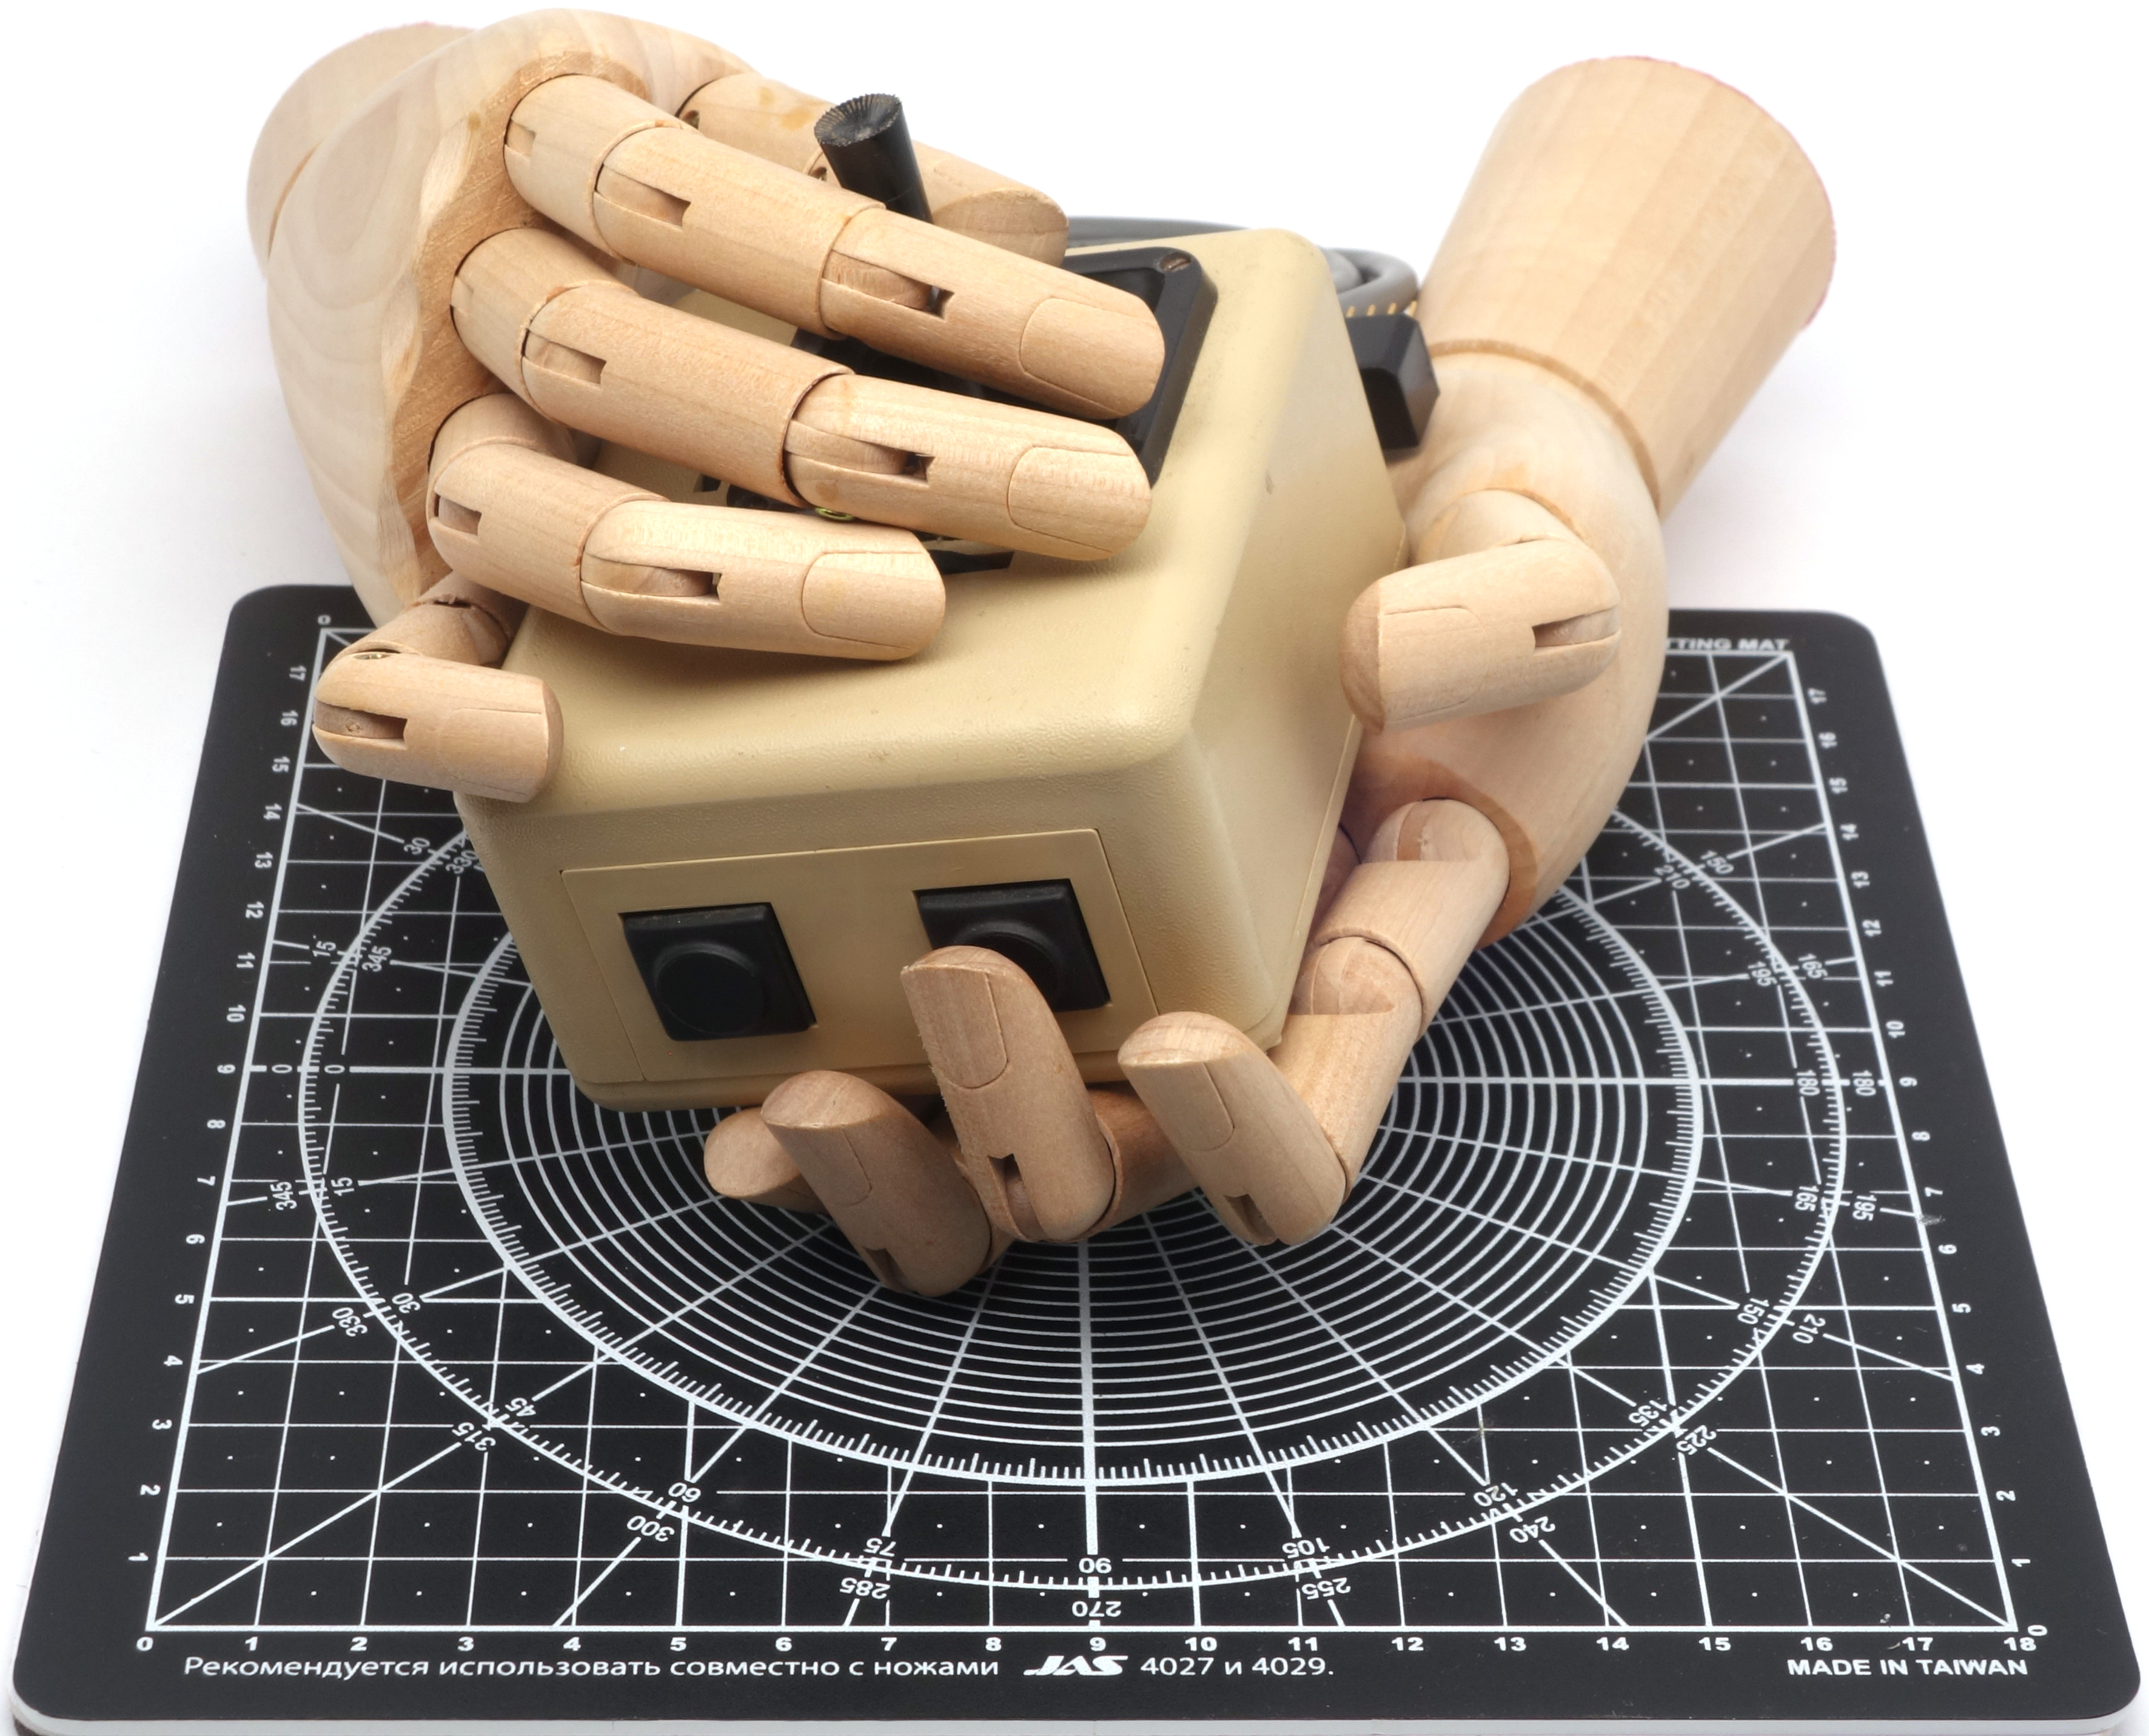
\includegraphics[scale=0.45]{1982_a2d_joystick_2001/hand2_30.jpg}
    \caption{A2D Joystick 2001 with a human hand model, held in hand}
    \label{fig:A2DJoystick2001TwoHands}
\end{figure}

However, as can be seen from the figure \ref{fig:A2DJoystick2001Hand}, tabletop use of the joystick is at least no less convenient when the fingers of one hand hold the body and press the buttons, while the fingers of the other hand control the stick.

\begin{figure}[h]
    \centering
    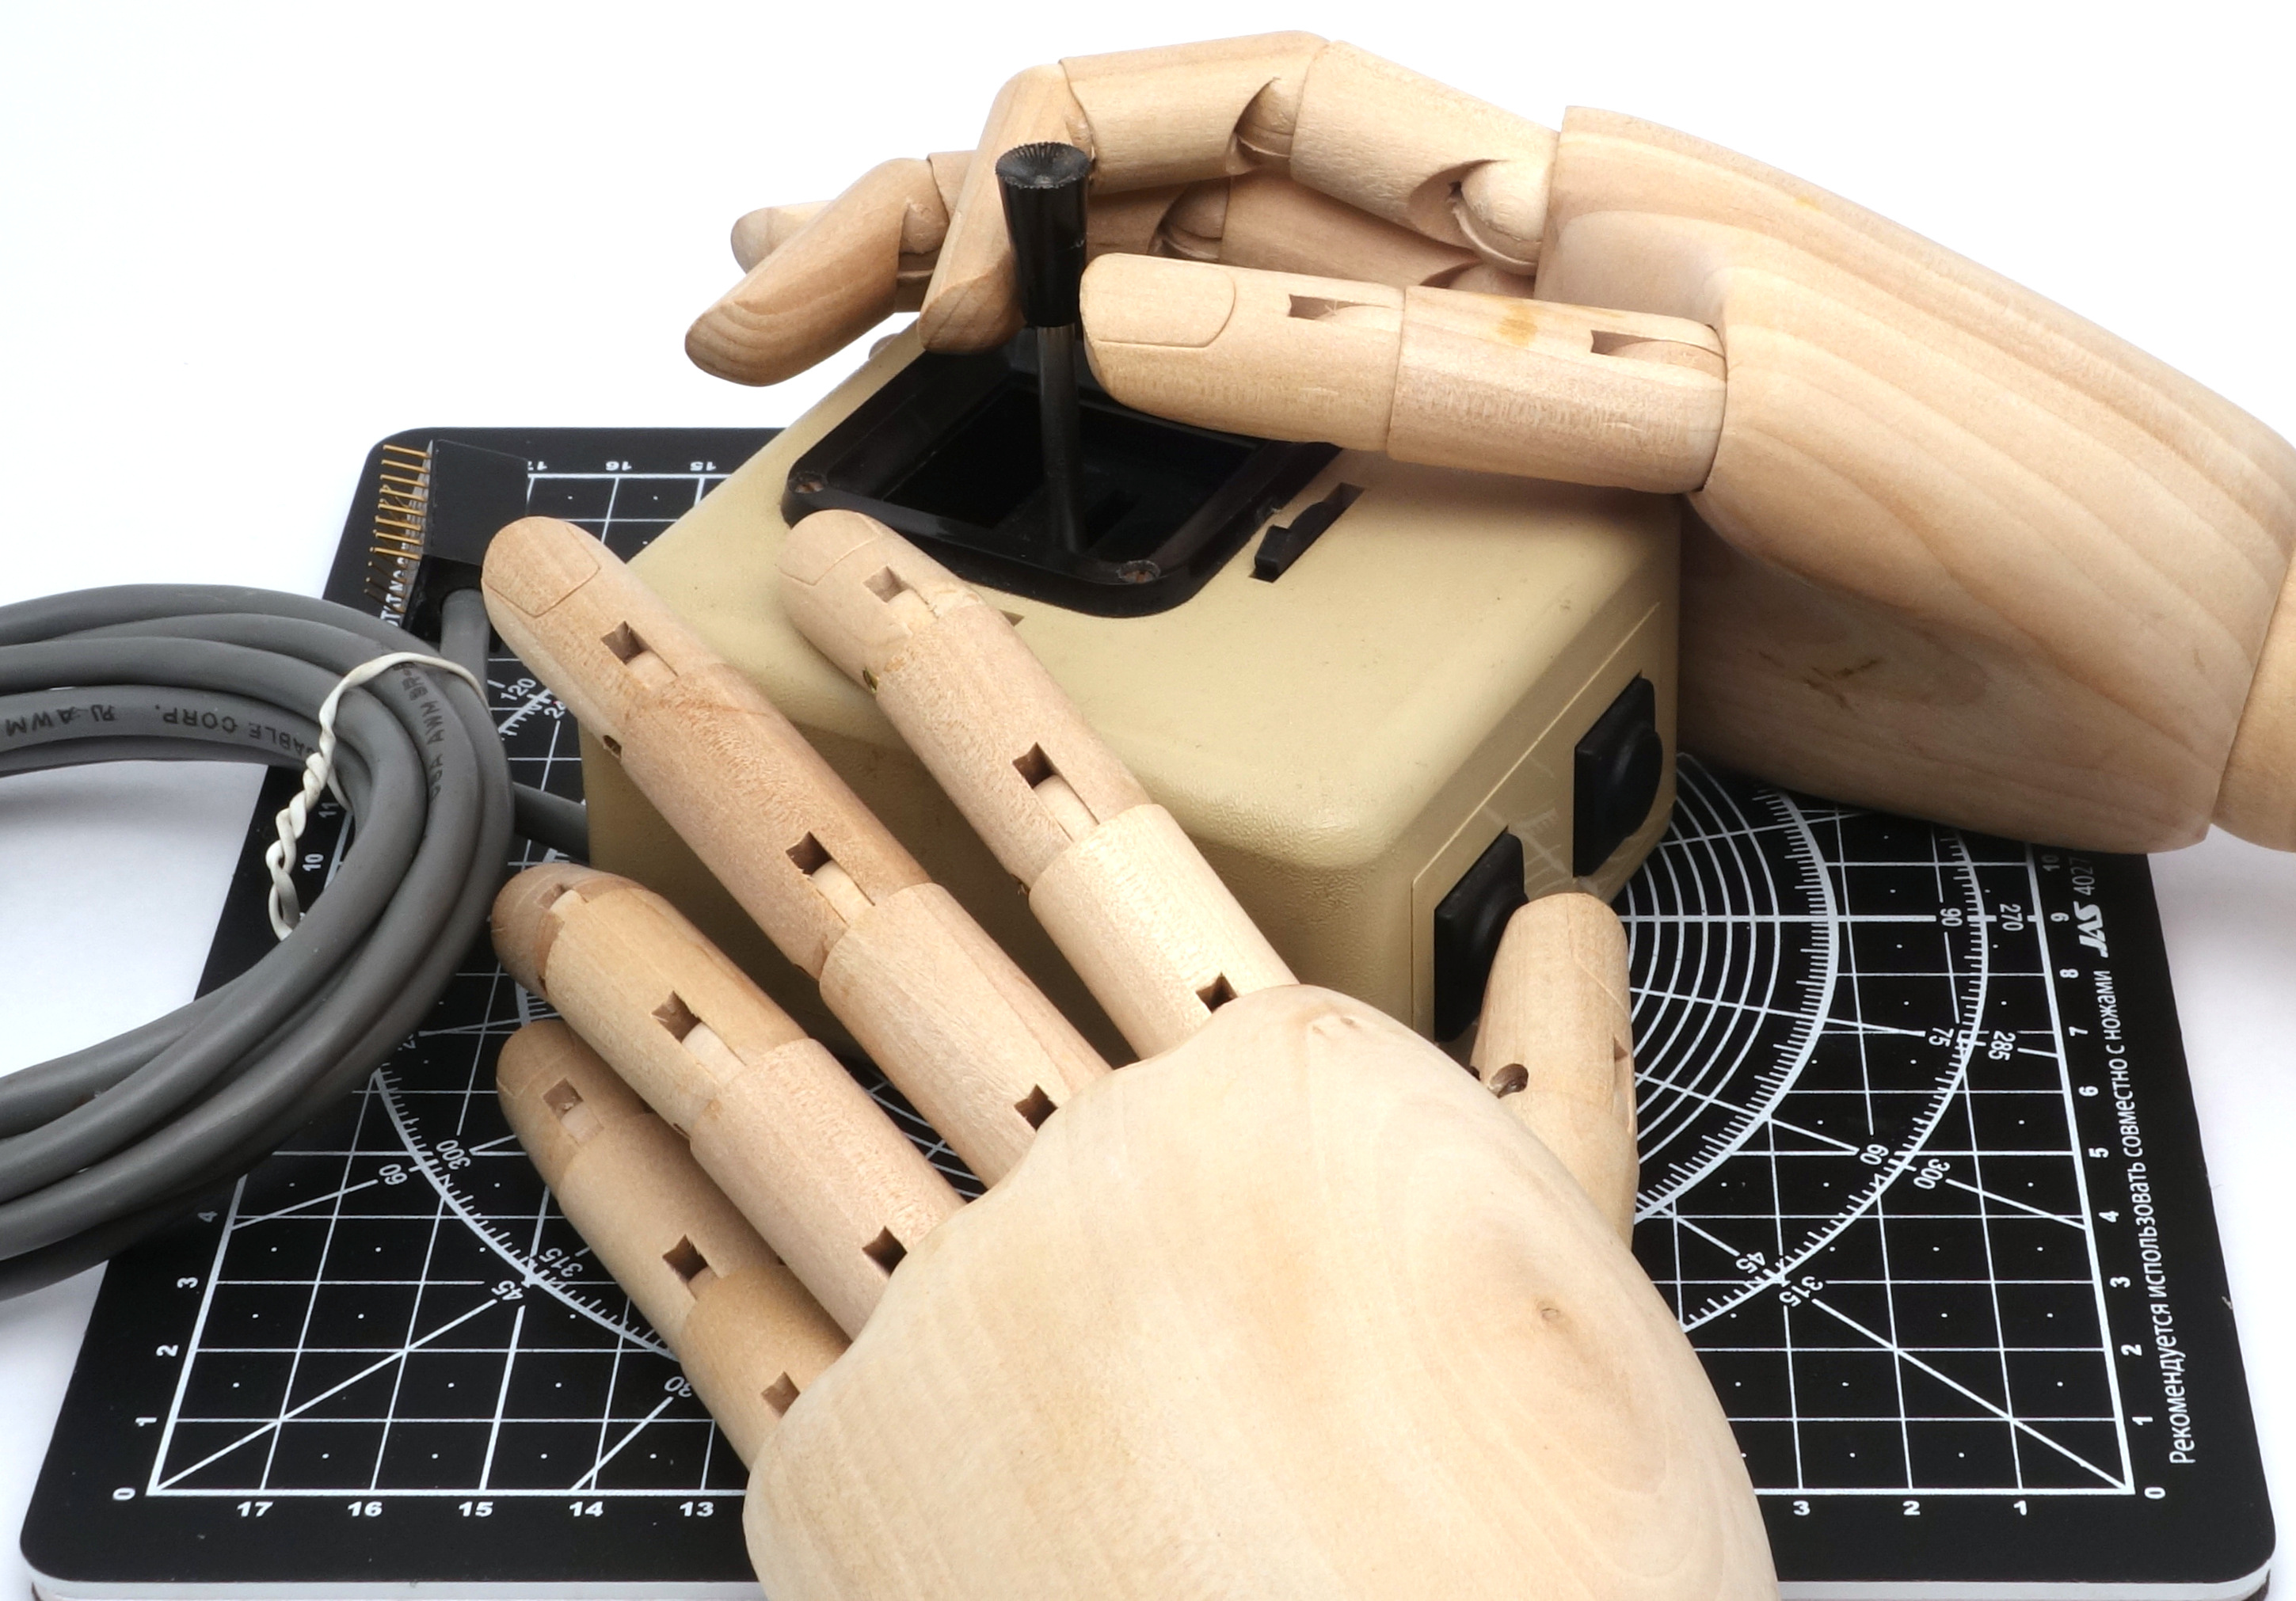
\includegraphics[scale=0.54]{1982_a2d_joystick_2001/hand3_30.jpg}
    \caption{A2D Joystick 2001 with a human hand model, tabletop use}
    \label{fig:A2DJoystick2001Hand}
\end{figure}

The stick handle from traditional cursor controlling joysticks used in a device designed primarily for gaming was somewhat disorienting for its target audience, but as noted in \cite{info_3}, being controlled with fingers (fig. \ref{fig:A2DJoystick2001Hand}) it didn't create significant issues in games. Same source also notes a big improvement in the buttons compared to the first model: they are large, with concave caps, ``have a very short travel distance, and provide excellent tactile and audible feedback''.

Same as in the first model, the joystick assembly, including the entire electromechanical unit, was proudly borrowed from R/C models remote controls. This relation was intentionally emphasized, mentioning ``precision open gimbal stick'' \cite{joustickAD}, ``developed for championship acrobatic R/C flying'' \cite{joystick81}. Reviewers mention its ``very smooth precise action'' \cite{a2d_paddles}.


\section*{Internal design}

The internal design of the joystick assembly is fairly standard, based on analog potentiometers, converting the deflection of the stick into a change in the electrical resistance (fig. \ref{fig:A2DJoystick2001Inside}). Like in the remote controls of R/C models, the sticks of A2D Joysticks are indeed placed on the metal gimbals actively advertised by the manufacturer. Also noteworthy is the use of a hand-routed PCB (instead of the hard-wired layout used in the previous model).

The device still has no screws to turn off self-centering mode of the stick (they were added in a subsequent model). One of the reviews proposed users who needed this to fix the situation manually by disassembling the joystick and removing the springs \cite{a2d_paddles}. 

\begin{figure}[h]
    \centering
    
\includegraphics[width=\textwidth]{1982_a2d_joystick_2001/inside_30.jpg}
    \caption{A2D Joystick 2001 disassembled}
    \label{fig:A2DJoystick2001Inside}
\end{figure}

\begin{thebibliography}{9}

\bibitem {a2d_paddles} J. Mazur. Hardtalk // Softalk, Vol.2, No 8, April 1982 -- p.58. \url{https://archive.org/details/softalkv2n08apr1982/page/57/mode/2up}

\bibitem {info_3} Ahl D.H. Joysticks, Paddles, and Game Port Extenders. Potentiometer Joysticks. A2D Joystick (2001) // Creative Computing, Vol.8, No 8, August 1982 -- p. 79. \url{https://archive.org/details/creativecomputing-1982-08/page/n79/mode/2up} % 82

\bibitem {a2d_answer} Porter H. Buttons Up, Thumbs Down // Softalk, Vol.2, No 10, June 1982. -- P. 24. \url{https://archive.org/details/softalkv2n10jun1982/page/24/mode/2up}

\bibitem {joustickAD} A2D Joystick 2001 (advertising) // Creative Computing, Vol.8, No 12, December 1982 -- p. 238 \url{https://archive.org/details/CreativeComputing1982-12/page/n231/mode/2up}

\bibitem{joystick81} Van Diver G., Love R. Apple II/III software directory. Vital Information, Inc., 1981. p. PR-21 \url{https://archive.org/details/vanlovesappleiii00gera/page/470/mode/1up?q=a2d+joystick}

\end{thebibliography}
\end{document}
